% \chapter[基于动态图元学习的噪声环境下小样本HRRP识别方法]{基于动态图元学习的噪声环境下小样本HRRP\protect\\ 识别方法}
\chapter[基于动态图元学习的噪声环境下小样本HRRP识别方法]{基于动态图元学习的噪声环境下小样本HRRP识别方法}
\label{chap:noise_robust}

\section{引言}
\label{sec:noise_intro}

实际部署中,HRRP信号固有的低信噪比特性是RATR面临的根本挑战,这一问题在小样本条件下尤为严峻,极易导致深度模型性能崩溃。尽管元学习为数据稀疏性提供了有力框架,但其标准范式往往缺乏对雷达特有复杂噪声环境的内禀鲁棒性。因此,如何在信号质量严重受损且样本极其有限的双重约束下,发展出具备噪声鲁棒性的元学习识别方法,是推动小样本RATR技术实用化的关键瓶颈。

本章聚焦于提升小样本HRRP识别在噪声环境下的鲁棒性。针对现有方法在低SNR和小样本双重约束下性能不足的问题,提出一种基于动态图元学习的噪声鲁棒识别方法HRRPGraphNet++。该方法的核心思想是将HRRP的距离单元关系显式建模为图结构,并创新性地引入动态图构建机制,使图连接能够根据输入HRRP样本自身的特性进行自适应调整。在此基础上,利用GNN提取对噪声扰动相对稳健的结构化特征表示。最后,将整个动态图学习模块嵌入到一个经过改进的、面向噪声鲁棒性改进的MAML++元学习框架中,赋予模型快速适应未知噪声环境并进行准确识别的能力。相较于传统依赖大量数据或噪声先验的方法,所提方法旨在利用元学习的快速适应性与动态图的自适应表示能力,构建兼具小样本学习能力与噪声鲁棒性的识别新范式。

本章的内容安排如下:第\ref{sec:noise_methodology}节首先对低信噪比条件下HRRP识别面临的问题进行分析,然后详细阐述所提出的基于动态图元学习的鲁棒识别方法,包括动态图构建策略、GNN表示学习模块、面向噪声鲁棒性的元学习框架设计以及整体算法流程;第\ref{sec:noise_experiments}节基于仿真实验结果,对所提方法的性能进行验证和分析,并与相关基线方法进行对比;第\ref{sec:noise_summary}节对本章的研究工作进行总结。

\section{基于动态图元学习的鲁棒识别方法}
\label{sec:noise_methodology}

本节详细介绍所提出的基于动态图元学习的噪声鲁棒小样本HRRP识别方法。首先分析低信噪比条件下HRRP识别面临的具体困难,然后阐述基于先验知识和注意力的动态图构建策略、图神经网络表示学习模块以及面向噪声鲁棒性的元学习框架设计,最后给出整体算法流程。

\subsection{低信噪比条件下HRRP识别问题分析}
\label{subsec:noise_challenge_analysis}

根据第二章的分析,实际观测到的HRRP样本 $p^{noisy}(r)$ 是理想目标信号 $s_o(t)$ 和噪声响应 $n_o(t)$ 经过脉冲压缩后相干叠加的幅度。噪声的存在对HRRP识别带来多方面困难:

首先,噪声会淹没或扭曲目标信号的精细结构。HRRP中的峰值对应于目标上的强散射中心,峰值的幅度、位置、宽度以及它们之间的相对关系是区分不同目标的关键信息。当SNR较低时,噪声的幅度可能与目标信号的幅度相当甚至更高,导致真实的散射中心峰值被淹没,或者出现由噪声引起的虚假峰值,使得从HRRP中提取稳定可靠的物理特征变得极为困难\upcite{du_noise_2016, liu_end--end_2022, liu_scnet_2024}。

其次,噪声会增加HRRP样本的类内差异(Intra-class Variance)。即使是同一目标在相同姿态角下的两次观测,由于噪声的随机性,其HRRP样本也可能呈现出显著差异。这种增大的类内差异使得学习一个能够将同类样本紧凑聚类的特征空间变得更加困难,尤其是在小样本条件下,模型看到的样本本就稀少,噪声引入的额外变化更容易导致模型混淆。

再次,噪声会干扰深度学习模型的训练过程。噪声的存在可能使得损失函数的梯度估计变得不稳定,模型收敛速度减慢,甚至收敛到局部最优解。更严重的是,在小样本条件下,模型可能会过度拟合训练样本中的噪声模式,而不是学习目标的本质特征,导致泛化能力严重下降。一个在干净数据上训练或元训练的模型,在面对含噪测试数据时性能往往会急剧恶化。

此外,真实雷达环境中的噪声往往具有复杂且时变的特性。噪声水平可能随系统工作状态、传播环境和距离变化。这要求识别模型不仅要对某种特定的噪声具有鲁棒性,更要具备对未知或变化的噪声环境的自适应能力。

因此,设计能够在低SNR、小样本条件下,并且对未知或变化的噪声具有鲁棒性和适应性的HRRP识别方法,是本章研究的核心目标。近期,Chen等\upcite{chen_hrrpgraphnet_2024}提出HRRPGraphNet指出基于图(Graph)的表示能够有效利用HRRP样本内的结构信息进行识别,然而其所采用的静态图构建方式,虽然融入了先验知识,但缺乏对不同噪声条件下信号特变化的自适应能力,限制了模型在噪声水平未知或变化时的泛化性能。基于以上观察,本章认为利用图结构来表示HRRP样本内部或样本之间的关系\upcite{defferrard_convolutional_2016, chen_hrrpgraphnet_2024, zhang_accelerating_2023},并通过动态调整图结构来适应不同的噪声特性,结合元学习的快速适应能力,是解决这一问题的有效途径。

\subsection{HRRP 样本的动态图构建策略}
\label{subsec:dynamic_graph_construction}

为了利用HRRP中蕴含的结构信息并增强对噪声的鲁棒性,本文将HRRP样本建模为图。具体地,对于一个长度为 $L$ 的离散HRRP样本 $\mathbf{p} = [p_1, \dots, p_L]^T$,将其视为一个包含 $L$ 个节点的图 $\mathcal{G} = (\mathcal{V}, \mathcal{E})$,其中节点集 $\mathcal{V} = \{v_1, \dots, v_L\}$ 对应于 $L$ 个距离单元,节点 $v_i$ 的初始特征可以设为该距离单元的幅度值 $p_i$ 或经过初始特征提取后的特征向量。图的关键在于如何定义节点之间的连接关系,即边集 $\mathcal{E}$ 或其对应的邻接矩阵 $\mathbf{A} \in \mathbb{R}^{L \times L}$。一个好的图结构应该能够反映距离单元之间有意义的物理或统计关联,并有助于GNN提取鲁棒特征。

考虑到HRRP的特性以及噪声的影响,本文创造性地提出一种混合动态图(Hybrid Dynamic Graph)构建策略,该策略结合了基于物理先验的静态连接和基于数据驱动的动态连接。

HRRP 数据本身蕴含着目标的结构信息,这种信息体现在距离单元之间的内在关联性上。根据雷达目标电磁散射的物理原理\upcite{Pathak199244, Song19971488, KELLER1962116},本文在HRRPGraphNet构建静态图方法的基础上,引入两个HRRP物理先验知识:

i.  局部相关性: 来自目标同一个局部结构部件或强散射区域的回波能量,经过脉冲压缩后,通常会分布在相邻的若干距离单元内。这意味着这些相邻或近距离的距离单元之间具有天然的强相关性。例如,一个强散射中心可能会展宽覆盖多个距离单元,这些单元应被视为一个整体或强关联体。

ii.  距离衰减效应: 物理上相距较远的距离单元所对应的目标部位,它们散射贡献之间的直接电磁相互作用通常较弱。因此,在HRRP上,相距较远的距离单元之间的相关性通常会随着它们之间距离的增加而减弱。

为了将这两种关于HRRP结构的基本物理先验知识(即局部相关性和距离衰减性)明确地编码到图模型中,作为一种独立于具体样本变化的结构化先验,即首先构建一个静态邻接矩阵 $\mathbf{A}^{\text{sta}}$。该矩阵旨在捕捉所有HRRP样本普遍共有的基础结构特性,为后续在噪声存在时稳定特征提取提供支撑\upcite{zhang_bayesian_2020, chen_target-attentional_2022}。基于此,定义静态连接权重 $A^{\text{sta}}_{ij}$ 为:
\begin{equation}
    A^{\text{sta}}_{ij} = \gamma \cdot \frac{1}{|i-j|+1} + (1-\gamma) \cdot \mathbb{I}(|i-j| \leq \delta)
    \label{eq:static_adjacency}
\end{equation}
其中,$|i-j|$ 是距离单元 $i$ 和 $j$ 之间的距离(索引差),$\mathbb{I}(\cdot)$ 是指示函数,$\delta$ 定义了一个局部连接窗口(例如,设为5,对应典型散射中心的展宽范围),$\gamma \in [0,1]$ 是一个平衡因子(例如,设为0.5),用于调节距离衰减项和局部窗口项的权重。这个静态图结构捕捉了HRRP信号中普遍存在的局部相关性和距离衰减特性,可以提供一种结构化的先验,有助于在噪声存在时稳定特征提取\upcite{zhang_bayesian_2020}。

然而,仅使用静态图结构无法完全捕捉HRRP中复杂且可能随样本变化的关联特性,也难以适应不同的噪声水平。例如,强散射中心之间的远程关联,或者噪声可能引入的虚假关联。为了使图结构能够根据输入样本自身的特性进行自适应调整,在光学领域工作的基础上\upcite{zhu_dynamic_2023, li_heterogeneous_2020, xu_traffic_2023, wang_attention-based_2022, hoang_dynamic-gtn_2022},本文设计了HRRP的动态图构建机制。该机制利用多头自注意力(Multi-Head Self-Attention)来学习节点之间的关系权重。

具体地,给定经过初始特征提取(例如,通过几层1D-CNN,详见下一节)得到的节点特征矩阵 $\mathbf{H} \in \mathbb{R}^{L \times d}$($d$为特征维度),计算查询(Query)、键(Key)、值(Value)矩阵。对于第 $h$ 个注意力头 ($h=1, \dots, N_{head}$),计算方式如下:
\begin{align}
    \mathbf{Q}_h &= \mathbf{H} \mathbf{W}_h^Q \in \mathbb{R}^{L \times d_h} \\
    \mathbf{K}_h &= \mathbf{H} \mathbf{W}_h^K \in \mathbb{R}^{L \times d_h} \\
    \mathbf{V}_h &= \mathbf{H} \mathbf{W}_h^V \in \mathbb{R}^{L \times d_h}
\end{align}
其中 $\mathbf{W}_h^Q, \mathbf{W}_h^K, \mathbf{W}_h^V \in \mathbb{R}^{d \times d_h}$ 是可学习的投影矩阵,$d_h = d / N_{head}$ 是每个头的维度。然后,计算注意力得分矩阵 $\mathbf{S}_h \in \mathbb{R}^{L \times L}$:
\begin{equation}
    \mathbf{S}_h = \frac{\mathbf{Q}_h \mathbf{K}_h^T}{\sqrt{d_h}}
    \label{eq:attention_scores}
\end{equation}
通过对注意力得分应用 Softmax 函数(按行),得到第 $h$ 个头的注意力权重矩阵 $\mathbf{A}_h^{\text{attn}} \in \mathbb{R}^{L \times L}$:
\begin{equation}
    \mathbf{A}_h^{\text{attn}} = \text{Softmax}(\mathbf{S}_h) = \text{Softmax}\left(\frac{\mathbf{Q}_h \mathbf{K}_h^T}{\sqrt{d_h}}\right)
    \label{eq:dynamic_adjacency_head}
\end{equation}
$\mathbf{A}_h^{\text{attn}}$ 的元素 $(i,j)$ 表示节点 $i$ 对节点 $j$ 的注意力权重。将所有头的注意力权重矩阵进行平均(也可以采用拼接或其他融合方式),得到最终的动态邻接矩阵 $\mathbf{A}^{\text{dyn}}$:
\begin{equation}
    \mathbf{A}^{\text{dyn}} = \frac{1}{N_{head}} \sum_{h=1}^{N_{head}} \mathbf{A}_h^{\text{attn}}
    \label{eq:dynamic_adjacency_final}
\end{equation}
$\mathbf{A}^{\text{dyn}}$ 是根据输入样本 $\mathbf{H}$ 动态计算得到的,能够捕捉数据中潜在的、可能非局部的、依赖于样本内容的关联结构\upcite{wu_feasibility_2024, bao_partial_2021, li_robust_2019, yang_time-aware_2023, dornaika_efficient_2017}。这种动态性有助于模型适应不同噪声水平下的信号特性,例如在高噪声下降低噪声节点的影响力,或在高信噪比下更关注强散射中心之间的关系。

为了结合静态先验和动态适应性,设计采用加权融合的方式得到最终的混合邻接矩阵 $\mathbf{A}^{\text{hybrid}}$:
\begin{equation}
    \mathbf{A}^{\text{hybrid}} = \lambda \cdot \mathbf{A}^{\text{sta}} + (1-\lambda) \cdot \mathbf{A}^{\text{dyn}}
    \label{eq:hybrid_adjacency}
\end{equation}
其中 $\lambda \in [0,1]$ 是一个超参数(或可学习参数),用于控制静态和动态成分的相对重要性。实验表明(见\ref{sec:noise_experiments}节),选择合适的 $\lambda$ (如 $\lambda=0.3$)可以获得比单独使用静态或动态图更好的性能。

最后,为了在GNN中稳定数值计算和信息传播\upcite{yu_enabling_2024, skryagin_graph_2024, cai_graphnorm_2021},对混合邻接矩阵进行对称归一化(Symmetric Normalization):
\begin{equation}
    \hat{\mathbf{A}} = \mathbf{D}^{-\frac{1}{2}} \mathbf{A}^{\text{hybrid}} \mathbf{D}^{-\frac{1}{2}}
    \label{eq:normalized_adjacency}
\end{equation}
其中 $\mathbf{D}$ 是 $\mathbf{A}^{\text{hybrid}}$ 的度矩阵(Degree Matrix),即 $D_{ii} = \sum_j A^{\text{hybrid}}_{ij}$ 且 $D_{ij}=0$ ($i \neq j$)。$\hat{\mathbf{A}}$ 将作为后续GNN层的传播矩阵。

通过这种混合动态图构建策略,将每个HRRP样本转换成一个既包含物理先验又具有数据自适应性的图表示,为GNN提取鲁棒特征奠定了基础。

\subsection{图神经网络表示学习模块}
\label{subsec:gnn_module}

在构建了图表示 $\mathcal{G} = (\mathcal{V}, \hat{\mathbf{A}})$ 之后,使用图神经网络(GNN)来学习节点的表示(Node Representations),并通过聚合节点表示得到整个HRRP图的表示(Graph Representation)用于最终的分类。本文设计的GNN架构主要包括初始特征提取、多层图卷积和全局图池化三个部分。

首先,需要为图中的每个节点(距离单元) $v_i$ 定义一个初始特征向量。直接使用原始HRRP幅度值 $p_i$ 作为初始特征可能信息量不足。因此,采用一个浅层的1D-CNN模块 $f_{\text{CNN}}$ 对原始HRRP向量 $\mathbf{p} \in \mathbb{R}^{L}$ 进行初始特征提取,得到节点初始特征矩阵 $\mathbf{H}^{(0)} \in \mathbb{R}^{L \times d_0}$:
\begin{equation}
    \mathbf{H}^{(0)} = f_{\text{CNN}}(\mathbf{p})
    \label{eq:initial_features}
\end{equation}
$f_{\text{CNN}}$ 通常包含几个卷积层、激活函数(如LeakyReLU)和归一化层(如BatchNorm)。例如,可以设计三层卷积块,通道数分别为16, 32, 64,最终输出维度 $d_0=64$。这个模块的作用是提取HRRP中的局部模式,并将原始的一维信号映射到一个更高维的特征空间,为后续的图卷积和动态图构建(需要输入 $\mathbf{H}$)提供更丰富的表示。

接着,堆叠 $T$ 层图卷积层(Graph Convolutional Layer, GC Layer)~\cite{kipf_semi-supervised_2017} 来进行节点特征的传播和更新。第 $t$ 层 ($t=0, \dots, T-1$) 的图卷积操作可以表示为:
\begin{equation}
    \mathbf{H}^{(t+1)} = \sigma\left(\hat{\mathbf{A}} \mathbf{H}^{(t)} \mathbf{W}^{(t)}\right)
    \label{eq:gcn_layer}
\end{equation}
其中 $\mathbf{H}^{(t)} \in \mathbb{R}^{L \times d_t}$ 是第 $t$ 层的节点特征矩阵($\mathbf{H}^{(0)}$ 是初始特征),$\mathbf{W}^{(t)} \in \mathbb{R}^{d_t \times d_{t+1}}$ 是该层可学习的权重矩阵,$\sigma(\cdot)$ 是非线性激活函数(如LeakyReLU)。$\hat{\mathbf{A}}$ 是式~(\ref{eq:normalized_adjacency}) 中计算得到的归一化邻接矩阵。这个操作可以理解为两步:首先,通过左乘 $\hat{\mathbf{A}}$,每个节点聚合其邻居节点(根据 $\hat{\mathbf{A}}$ 定义的连接和权重)的特征;然后,通过右乘 $\mathbf{W}^{(t)}$ 并应用激活函数 $\sigma$,对聚合后的特征进行线性变换和非线性映射,得到该层输出的新特征。通过堆叠 $T$ 层GCN,节点能够聚合到来自其 $T$-hop 邻域的信息,从而学习到更高阶的结构特征。在本文的实现中,设置 $T=3$。在每层GCN后,还加入了BatchNorm和Dropout来提高训练稳定性和泛化能力:
\begin{equation}
    \mathbf{H}^{(t+1)} = \text{Dropout}\left(\text{BN}\left(\sigma\left(\hat{\mathbf{A}} \mathbf{H}^{(t)} \mathbf{W}^{(t)}\right)\right); \text{p}_{drop}\right)
    \label{eq:gcn_layer_full}
\end{equation}
其中 $\text{p}_{drop}=0.1$ 为Dropout概率。

经过 $T$ 层图卷积后,得到最终的节点特征矩阵 $\mathbf{H}^{(T)} \in \mathbb{R}^{L \times d_T}$。为了得到代表整个HRRP图的单一向量表示,需要进行图池化(Graph Pooling)操作。简单的全局平均池化或最大池化可能会丢失重要信息或对噪声敏感。因此,采用全局注意力池化(Global Attention Pooling)~\upcite{velickovic_graph_2018},它能够根据节点特征的重要性自适应地计算加权和。首先,计算每个节点 $v_i$ 的注意力得分 $e_i$:
\begin{equation}
    e_i = \mathbf{w}_{att}^T \sigma_{att}(\mathbf{W}_{att} \mathbf{h}_i^{(T)} + \mathbf{b}_{att})
    \label{eq:attention_score_node}
\end{equation}
其中 $\mathbf{h}_i^{(T)}$ 是 $\mathbf{H}^{(T)}$ 的第 $i$ 行,$\mathbf{W}_{att}, \mathbf{b}_{att}, \mathbf{w}_{att}$ 是可学习的注意力网络参数,$\sigma_{att}$ 是激活函数(如Tanh或LeakyReLU)。然后,通过Softmax函数将得分归一化为注意力权重 $\alpha_i$:
\begin{equation}
    \alpha_i = \frac{\exp(e_i)}{\sum_{j=1}^L \exp(e_j)}
    \label{eq:attention_weight_node}
\end{equation}
最后,计算所有节点特征的加权和,得到图级别的表示向量 $\mathbf{z} \in \mathbb{R}^{d_T}$:
\begin{equation}
    \mathbf{z} = \sum_{i=1}^L \alpha_i \mathbf{h}_i^{(T)}
    \label{eq:graph_representation}
\end{equation}
这个图表示 $\mathbf{z}$ 捕捉了整个HRRP样本的关键信息,并能对噪声具有一定的鲁棒性,因为它通过注意力机制侧重于更重要的节点特征。$\mathbf{z}$ 将作为最终分类器的输入。

\subsection{面向噪声鲁棒性的元学习框架设计}
\label{subsec:meta_learning_noise_robust}

为使本文提出的动态图神经网络模型能够在小样本、低信噪比条件下有效工作,并具备对未知或变化噪声水平的适应能力,我们将其嵌入到一个经过改进的元学习框架中。本文思路是选择基于优化的元学习范式,特别是以MAML为基础进行改进,其核心优势在于直接优化模型的快速适应能力。面对噪声这一关键挑战,模型需要在接触到新任务的少量支持样本时,能迅速调整自身以适应当前特定的噪声特性。基于优化的元学习通过内循环梯度更新显式地模拟了这一适应过程,旨在学习一个对这种快速调整最优化的模型起点,这使其成为构建自适应噪声鲁棒性识别器的天然选择。 为此,本章对标准MAML框架进行了几项关键改进,以增强其在处理复杂HRRP数据和噪声环境下的鲁棒性与适应效率。

HRRPGraphNet++的元学习框架遵循第二章介绍的S/Q Training范式。在元训练阶段,从基础数据集 $D_{base}$ 中采样大量的 $N$-way $K$-shot 任务 $\mathcal{T}_i = (\mathcal{S}_i, \mathcal{Q}_i)$。虽然元训练任务本身可能采样自干净数据或设定在某一固定噪声水平,但其核心目标是学习一种通用的适应机制。通过在大量不同类别组合的任务上进行训练,模型被期望掌握一种元知识,使其在元测试阶段,即使面对含有未知或不同水平噪声(如式~(\ref{eq:hrrp_noisy})所示)的新任务支持集 $\mathcal{S}_{new}$ 时,也能通过内循环的快速调整,有效提取判别信息并进行准确分类,从而实现对噪声变化的鲁棒泛化。HRRPGraphNet++采用类似MAML++~\cite{antoniou_how_2018, yao_model-agnostic_2021, zhou_task_2021, raghu_rapid_2020}的改进策略来优化元学习过程,这些改进对于处理复杂的HRRP数据和噪声尤其重要:

i.  多步内循环更新(Multi-step Inner Loop Updates):在任务适应阶段(内循环),不只进行一步梯度更新,而是进行 $U$ 步(例如 $U=5$)更新,以获得更充分的任务适应:
    \begin{equation}
        \theta_i^{(u+1)} = \theta_i^{(u)} - \alpha^{(u)} \nabla_{\theta_i^{(u)}} \mathcal{L}_{\mathcal{S}_i}(\theta_i^{(u)}), \quad u=0, \dots, U-1
        \label{eq:multi_step_inner_update}
    \end{equation}
    其中 $\theta_i^{(0)} = \theta$ 是元参数。

ii.  多步损失优化(Multi-step Loss Optimization):在元更新阶段(外循环),不仅仅基于最后一步适应后的参数 $\theta_i^{(U)}$ 在查询集上的损失进行优化,而是利用所有 $U$ 步适应过程中的中间参数 $\theta_i^{(u)}$ ($u=1, \dots, U$) 在查询集上的损失的加权和作为元目标。这为元参数的更新提供了更丰富、更平滑的梯度信号:
    \begin{equation}
        \mathcal{L}_{\mathcal{T}_i}^{meta} = \sum_{u=1}^{U} w_u \mathcal{L}_{\mathcal{Q}_i}(\theta_i^{(u)})
        \label{eq:multi_step_loss}
    \end{equation}
    其中 $w_u$ 是第 $u$ 步损失的权重(例如,可以随 $u$ 增大而增大,如 $w_u \propto u$ 或指数增长,使得后期适应结果更重要)。元更新的目标变为 $\min_{\theta} \mathbb{E}_{\mathcal{T}_i} [\mathcal{L}_{\mathcal{T}_i}^{meta}]$。

iii.  层级学习率(Layer-wise Learning Rates):考虑到深度神经网络中不同层学习特征的抽象程度不同,以及它们对任务适应的敏感度可能不同,为内循环的梯度更新引入层级(或更细粒度的,如参数级)学习率 $\alpha^{(u)}_l$。例如,可以让靠近输出的层(如分类层)具有较大的学习率以便快速调整决策边界,而让靠近输入的层(如特征提取层、图卷积层)具有较小的学习率以保持学到的通用特征表示的稳定性。这可以通过将学习率向量 $\boldsymbol{\alpha}^{(u)}$ 与梯度进行逐元素相乘来实现:
    \begin{equation}
        \theta_i^{(u+1)} = \theta_i^{(u)} - \boldsymbol{\alpha}^{(u)} \odot \nabla_{\theta_i^{(u)}} \mathcal{L}_{\mathcal{S}_i}(\theta_i^{(u)})
        \label{eq:layerwise_lr_update}
    \end{equation}
    学习率 $\boldsymbol{\alpha}^{(u)}$ 本身也可以作为元参数进行学习(如Meta-SGD\upcite{li_meta-sgd_2017}),或者根据经验为不同层设置不同的固定比率。我们发现在HRRP识别中,让图卷积层比初始CNN特征提取层具有稍高的学习率有助于模型更好地适应图结构的变化。

iv.  任务级批归一化统计量(Task-Level Batch Normalization Statistics):批归一化(BatchNorm, BN)层在深度学习中广泛用于加速训练和提高泛化能力。但在元学习中,BN层的运行统计量(均值和方差)的处理需要特别注意。如果在元训练时使用全局统计量,可能无法很好地适应新任务的数据分布;如果在内循环中完全重新计算统计量,可能导致训练不稳定。HRRPGraphNet++采用一种折中方案,即在内循环的每一步更新中,使用当前任务支持集 $\mathcal{S}_i$ 的数据来计算BN层的均值和方差,但在元更新时,不通过这些统计量的计算过程进行梯度反向传播(即将其视为固定的)。这有助于模型适应每个任务的特征分布变化(可能由噪声引起),同时保持元优化的稳定性。

通过将动态图构建模块、GNN表示学习模块集成到这个经过改进的元学习框架中,并在包含不同噪声水平的任务上进行元训练,本方法最终得到的元参数 $\theta^*$ 能够编码一种对噪声具有鲁棒性、能够快速适应新类别和小样本含噪数据的HRRP识别能力。

\subsection{整体方法流程与算法伪代码}
\label{subsec:algorithm}

我们将所提出的基于动态图元学习的噪声鲁棒小样本HRRP识别方法HRRPGraphNet++的整体流程总结在算法~\ref{alg:meta_training}(元训练阶段)和算法~\ref{alg:meta_testing}(元测试阶段)中。

\begin{figure}[h]
    \centering
    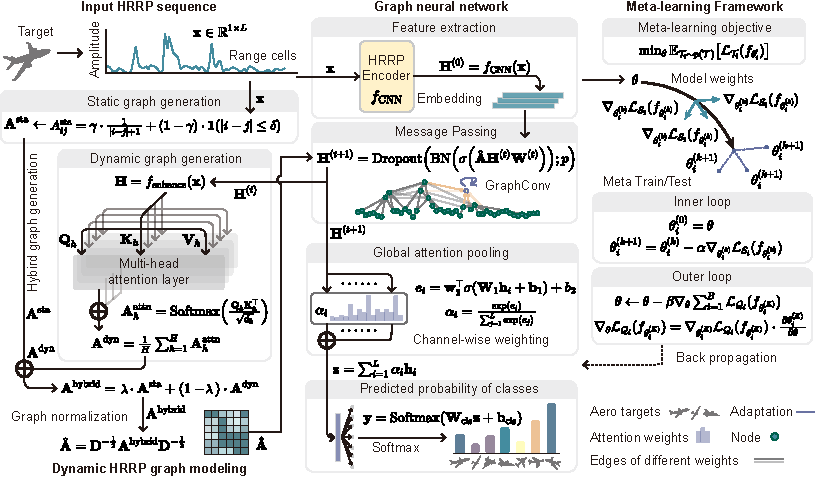
\includegraphics[width=\linewidth]{figures/method1.pdf} % 使用与原文相同的图
    % \fbox{图 3.1: 12类飞机HRRP样本示例 (占位符,同原文 Figure 2)}
    \caption{所提HRRPGraphNet++整体方法流程示意图}
    \label{fig:dataset_chap3}
\end{figure}

在元训练阶段(算法~\ref{alg:meta_training}),模型通过在大量从基类别 $C_{base}$ 采样并可能加入不同噪声的模拟任务 $\mathcal{T}_i=(\mathcal{S}_i, \mathcal{Q}_i)$ 上进行学习,来优化元参数 $\theta$(包括CNN特征提取器、动态图注意力网络、GNN以及最终分类器的参数)。对于每个任务,首先基于共享的元参数 $\theta$ 初始化任务特定参数 $\theta_i^{(0)}$。然后,在内循环中,使用支持集 $\mathcal{S}_i$ 进行 $U$ 步梯度更新,得到适应后的参数 $\theta_i^{(u)}$ ($u=1, \dots, U$)。在每一步更新中,需要根据当前节点特征计算动态图邻接矩阵 $\mathbf{A}^{\text{dyn}}$,并与静态矩阵 $\mathbf{A}^{\text{sta}}$ 融合得到 $\mathbf{A}^{\text{hybrid}}$,再进行归一化得到 $\hat{\mathbf{A}}$,然后通过GNN前向传播计算损失 $\mathcal{L}_{\mathcal{S}_i}(\theta_i^{(u)})$,最后使用层级学习率 $\boldsymbol{\alpha}^{(u)}$ 更新参数。内循环结束后,在外循环中,计算查询集 $\mathcal{Q}_i$ 在所有 $U$ 步适应后的参数下的加权损失 $\mathcal{L}_{\mathcal{T}_i}^{meta}$。最后,基于一批任务的平均元损失 $\sum_i \mathcal{L}_{\mathcal{T}_i}^{meta}$ 来计算元梯度 $\nabla_\theta (\sum_i \mathcal{L}_{\mathcal{T}_i}^{meta})$(可能使用一阶近似),并使用元学习率 $\beta$ 更新元参数 $\theta$。这个过程不断重复直到收敛。

% ----- Replacement for Algorithm 3.1 (alg:meta_training) -----
\begin{algorithm}[htbp] % Use placement specifier like the example
\caption{HRRPGraphNet++ 元训练阶段}
\label{alg:meta_training}
\begin{algorithmic}[1] % Use [1] for line numbers like the example
    \REQUIRE 任务分布 $p(\mathcal{T})$,内循环学习率 $\boldsymbol{\alpha}^{(u)}$ ($u=0..U-1$),元学习率 $\beta$,损失权重 $w_u$ ($u=1..U$)
    \ENSURE 优化后的元参数 $\theta^*$
    \STATE 初始化元参数 $\theta$
    \WHILE{未收敛}
        \STATE 采样一批任务 $\{\mathcal{T}_i = (\mathcal{S}_i, \mathcal{Q}_i)\}_{i=1}^{B_{task}} \sim p(\mathcal{T})$ % \Comment{任务可能包含不同噪声水平} % Standard comment if needed
        \STATE 初始化元梯度 $\nabla_\theta L_{meta} = 0$
        \FOR{每个任务 $\mathcal{T}_i$}
            \STATE $\theta_i^{(0)} \leftarrow \theta$
            \FOR{$u = 0$ to $U-1$} %\Comment{内循环:任务适应}
                \STATE 令 $\mathbf{p}_s \in \mathcal{S}_i$
                \STATE $\mathbf{H}^{(0)} \leftarrow f_{\text{CNN}}(\mathbf{p}_s; \theta_i^{(u)})$ %\Comment{初始特征提取}
                \STATE $\mathbf{A}^{\text{dyn}} \leftarrow \text{Attention}(\mathbf{H}^{(0)}; \theta_i^{(u)})$ %\Comment{计算动态图}
                \STATE $\mathbf{A}^{\text{hybrid}} \leftarrow \lambda \mathbf{A}^{\text{sta}} + (1-\lambda) \mathbf{A}^{\text{dyn}}$
                \STATE $\hat{\mathbf{A}} \leftarrow \mathbf{D}^{-\frac{1}{2}} \mathbf{A}^{\text{hybrid}} \mathbf{D}^{-\frac{1}{2}}$
                \STATE $\mathbf{z} \leftarrow \text{GNN}(\mathbf{H}^{(0)}, \hat{\mathbf{A}}; \theta_i^{(u)})$ %\Comment{GNN表示学习与池化}
                \STATE $\mathcal{L}_{\mathcal{S}_i}(\theta_i^{(u)}) \leftarrow \text{Loss}( \text{Classifier}(\mathbf{z}; \theta_i^{(u)}), \text{labels}(\mathcal{S}_i) )$
                \STATE $\theta_i^{(u+1)} \leftarrow \theta_i^{(u)} - \boldsymbol{\alpha}^{(u)} \odot \nabla_{\theta_i^{(u)}} \mathcal{L}_{\mathcal{S}_i}(\theta_i^{(u)})$ %\Comment{使用任务级BN统计量}
            \ENDFOR % End Inner For
            \STATE 计算元损失 $\mathcal{L}_{\mathcal{T}_i}^{meta} = \sum_{u=1}^{U} w_u \mathcal{L}_{\mathcal{Q}_i}(\theta_i^{(u)})$ %\Comment{外循环:计算元损失}
            \STATE 累加元梯度 $\nabla_\theta L_{meta} \leftarrow \nabla_\theta L_{meta} + \nabla_\theta \mathcal{L}_{\mathcal{T}_i}^{meta}$ %\Comment{可能使用一阶近似}
        \ENDFOR % End Task For
        \STATE 更新元参数 $\theta \leftarrow \theta - \beta \frac{1}{B_{task}} \nabla_\theta L_{meta}$ %\Comment{元更新}
    \ENDWHILE % End While
    \STATE $\theta^* \leftarrow \theta$
\end{algorithmic}
\end{algorithm}

% ----- Replacement for Algorithm 3.2 (alg:meta_testing) -----
\begin{algorithm}[htbp]
\caption{HRRPGraphNet++ 元测试阶段}
\label{alg:meta_testing}
\begin{algorithmic}[1]
    \REQUIRE 优化后的元参数 $\theta^*$, 新任务 $\mathcal{T}_{new} = (\mathcal{S}_{new}, \mathcal{Q}_{new})$
    \ENSURE 预测结果 $\{\hat{y}_q\}$ for all $\mathbf{p}_q \in \mathcal{Q}_{new}$
    \STATE $\theta_{new}^{(0)} \leftarrow \theta^*$ %\Comment{使用元参数初始化}
    \FOR{$u = 0$ to $U-1$} %\Comment{任务适应}
        \STATE 令 $\mathbf{p}_s \in \mathcal{S}_{new}$
        \STATE $\mathbf{H}^{(0)} \leftarrow f_{\text{CNN}}(\mathbf{p}_s; \theta_{new}^{(u)})$
        \STATE $\mathbf{A}^{\text{dyn}} \leftarrow \text{Attention}(\mathbf{H}^{(0)}; \theta_{new}^{(u)})$
        \STATE $\mathbf{A}^{\text{hybrid}} \leftarrow \lambda \mathbf{A}^{\text{sta}} + (1-\lambda) \mathbf{A}^{\text{dyn}}$
        \STATE $\hat{\mathbf{A}} \leftarrow \mathbf{D}^{-\frac{1}{2}} \mathbf{A}^{\text{hybrid}} \mathbf{D}^{-\frac{1}{2}}$
        \STATE $\mathbf{z} \leftarrow \text{GNN}(\mathbf{H}^{(0)}, \hat{\mathbf{A}}; \theta_{new}^{(u)})$
        \STATE $\mathcal{L}_{\mathcal{S}_{new}}(\theta_{new}^{(u)}) \leftarrow \text{Loss}( \text{Classifier}(\mathbf{z}; \theta_{new}^{(u)}), \text{labels}(\mathcal{S}_{new}) )$
        \STATE $\theta_{new}^{(u+1)} \leftarrow \theta_{new}^{(u)} - \boldsymbol{\alpha}^{(u)} \odot \nabla_{\theta_{new}^{(u)}} \mathcal{L}_{\mathcal{S}_{new}}(\theta_{new}^{(u)})$ %\Comment{使用任务级BN统计量}
    \ENDFOR
    \STATE % Use empty \STATE for a blank line if needed, or \Statex if available
    %\STATE \Comment{对查询样本进行预测} % Use \Comment if needed
    \STATE Initialize $Y_{pred} = [~]$
    \FOR{each $\mathbf{p}_q \in \mathcal{Q}_{new}$}
        \STATE $\mathbf{H}_q^{(0)} \leftarrow f_{\text{CNN}}(\mathbf{p}_q; \theta_{new}^{(U)})$
        \STATE $\mathbf{A}_q^{\text{dyn}} \leftarrow \text{Attention}(\mathbf{H}_q^{(0)}; \theta_{new}^{(U)})$
        \STATE $\mathbf{A}_q^{\text{hybrid}} \leftarrow \lambda \mathbf{A}^{\text{sta}} + (1-\lambda) \mathbf{A}_q^{\text{dyn}}$
        \STATE $\hat{\mathbf{A}}_q \leftarrow \mathbf{D}_q^{-\frac{1}{2}} \mathbf{A}_q^{\text{hybrid}} \mathbf{D}_q^{-\frac{1}{2}}$
        \STATE $\mathbf{z}_q \leftarrow \text{GNN}(\mathbf{H}_q^{(0)}, \hat{\mathbf{A}}_q; \theta_{new}^{(U)})$
        \STATE $\hat{y}_q \leftarrow \arg\max (\text{Classifier}(\mathbf{z}_q; \theta_{new}^{(U)}))$
        \STATE Append $\hat{y}_q$ to $Y_{pred}$
    \ENDFOR
\end{algorithmic}
\end{algorithm}
在元测试阶段(算法~\ref{alg:meta_testing}),模型面对一个来自新类别 $C_{novel}$ 的新任务 $\mathcal{T}_{new} = (\mathcal{S}_{new}, \mathcal{Q}_{new})$。首先使用元训练得到的优化后的元参数 $\theta^*$ 来初始化模型 $\theta_{new}^{(0)}$。然后,完全按照元训练内循环的方式,使用新任务的支持集 $\mathcal{S}_{new}$ 进行 $U$ 步梯度更新,得到针对该新任务适应后的参数 $\theta_{new}^{(U)}$。最后,使用适应后的模型 $f_{\theta_{new}^{(U)}}$ 对查询集 $\mathcal{Q}_{new}$ 中的样本进行预测,得到识别结果 $\hat{y}_{query}$。这个过程模拟了模型在遇到新类别、只有少量样本的情况下快速学习并进行识别的能力。

\section{实验设计及结果分析}
\label{sec:noise_experiments}

为了验证所提出的HRRPGraphNet++方法的有效性,特别是在小样本和噪声环境下的性能,本章进行了一系列仿真实验。本节将详细介绍实验设置、所用数据集、评估指标、对比方法以及实验结果与分析。

数据集设定方面,所有实验均在一个广泛使用的飞机电磁仿真数据集上进行\upcite{chen_hrrpgraphnet_2024, liu_prior-knowledge-guided_2024, liu_scnet_2024, liu_multi-polarization_2021, liu_attribute-informed_2025}。该数据集包含了12种不同类型的飞机模型(EA-18G、EP-3E、F2、F15、F16、F18、F22、F35、Global Hawk、Mirage-2000、Predator Drone、IDF)在X波段(9.5-10.5 GHz,步进10MHz)下的仿真雷达回波数据。数据覆盖了俯仰角75°至105°(步长3°)和方位角0°至60°(步长0.05°)的范围,并包含四种极化模式(HH、HV、VH、VV)。在本章实验中,主要使用HH极化模式下,固定俯仰角90°的数据构建噪声条件小样本HRRP仿真数据集。对于每个飞机类型,可得到一个包含1201个不同方位角样本的HRRP序列,每个HRRP样本包含1000个距离单元。图~\ref{fig:dataset_chap3}展示了数据集中12类目标在某个特定角度下的HRRP样本示例。为了进行小样本学习实验,将这12类飞机按照类别1:1随机划分为训练集(包含$C_{base}=6$个类别)和测试集(包含$C_{novel}=6$个类别),确保训练集和测试集类别不重叠。为了模拟噪声环境,在元训练和元测试的任务构建阶段,向原始的干净HRRP样本中添加高斯白噪声,使得样本的SNR在[-5dB, 0dB, 5dB, 10dB, 15dB, 20dB]内变化,为模型评估构建了对应的噪声元测试集。

% --- 数据集示意图占位符 ---
\begin{figure}[h!]
    \centering
    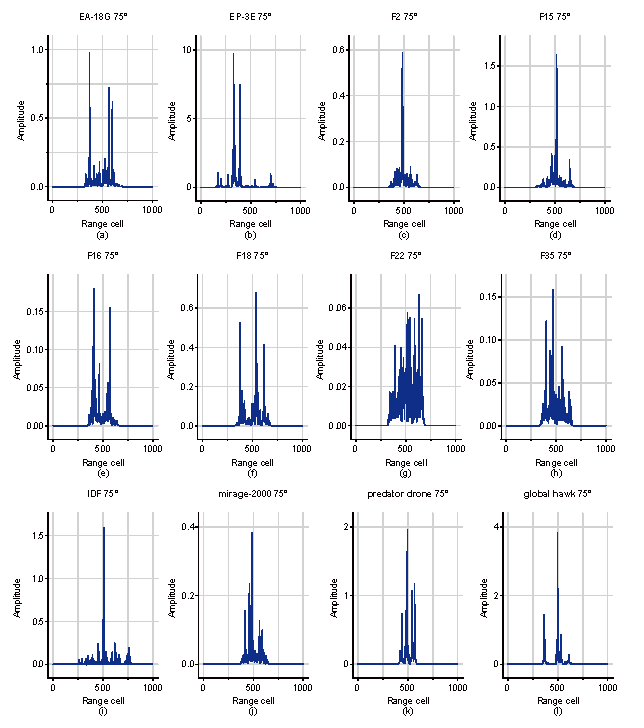
\includegraphics[width=\linewidth]{figures/hrrp_samples.pdf} % 使用与原文相同的图
    % \fbox{图 3.1: 12类飞机HRRP样本示例 (占位符,同原文 Figure 2)}
    \caption{实验数据集中12类飞机目标在俯仰角90°,方位角0.15°下的HRRP样本}
    \label{fig:dataset_chap3}
\end{figure}

实验设置上,所有模型均使用PyTorch 2.2.0框架实现,并在配置3*NVIDIA RTX A4000 GPU、2*Intel(R) Xeon(R) Bronze 3204 CPU @ 1.90GHz、64GB RAM的服务器上进行训练和测试,如不特别说明,后续章节均遵照此配置进行。采用Adam优化器进行元参数 $\theta$ 的更新,初始元学习率 $\beta$ 设置为5e-4,权重衰减为1e-2。元训练过程采用的任务批次大小(BS of Tasks)为4,最大训练轮数(Epochs)为300,并使用早停(Early Stopping)策略(Patience=100)防止过拟合。内循环适应步数 $U$ 设为5。内循环学习率 $\boldsymbol{\alpha}^{(u)}$ 采用层级设置,并随步数 $u$ 衰减,具体而言,对于图卷积层,初始学习率较高(0.006),对于CNN特征提取层较低(0.004),并逐步减小至最后一步(0.001)。多步损失权重 $w_u$ 采用[0.1, 0.2, 0.3, 0.4, 1.0]的设置。

为验证所提HRRPGraphNet++的性能,本文选择了一系列有代表性的方法进行性能比较,包括:传统的RATR方法,如主成分分析结合支持向量机(PCA-SVM)\upcite{liu_experimental_2020}和模板匹配(TemplateMatcher)\upcite{cui_template_2022};基于标准深度学习的方法,如1D-CNN\upcite{song_radar_2019}和LSTM\upcite{jithesh_lstm_2017}(这些模型在小样本数据上进行直接训练);基于图神经网络的方法,如图卷积网络(Graph Convolutional Network,GCN)\upcite{kipf_semi-supervised_2017}和图注意力网络(Garph Attention Network,GAT)\upcite{velickovic_graph_2018}(将HRRP视为图,使用固定邻接矩阵);通用的元学习方法,如MAML\upcite{finn_model-agnostic_2017}, MAML++\upcite{antoniou_how_2018}, ANIL\upcite{aniruddh_anil_2020}, Meta-SGD\upcite{li_meta-sgd_2017}(采用1D-Conv64F作为主干);以及作者之前提出的仅使用静态图的HRRPGraphNet~\cite{chen_hrrpgraphnet_2024}。所有对比方法均在相同的训练、测试划分和任务设置下进行评估。

主要的评估指标是小样本分类准确率(Accuracy)。对于元测试阶段的每个 $N$-way $K$-shot 任务 $\mathcal{T}_i = (\mathcal{S}_i, \mathcal{Q}_i)$,模型首先使用支持集 $\mathcal{S}_i$ 进行适应得到参数 $\theta_i^{(U)}$,然后在查询集 $\mathcal{Q}_i$ 上进行预测,计算准确率:
\begin{equation}
    \text{Acc}(\mathcal{T}_i) = \frac{1}{|\mathcal{Q}_i|} \sum_{(\mathbf{x},y) \in \mathcal{Q}_i} \mathbb{I}(f_{\theta_i^{(U)}}(\mathbf{x}) = y)
    \label{eq:accuracy_metric}
\end{equation}
为了获得统计上可靠的结果,对每个实验设置(如 $N$-way $K$-shot,特定SNR)随机生成600个测试任务,并报告这些任务准确率的平均值 $\overline{\text{Acc}}$。在本章的实验中,我们主要关注 $N=3$ 的情况,即 3-way $K$-shot 问题。

首先,本章比较了所提出的HRRPGraphNet++方法与其他基线方法在不同 $K$ 值(1-shot, 5-shot, 20-shot)下的平均识别准确率,实验在相对较高的信噪比(20dB)下进行。结果如表~\ref{tab:fewshot_comparison_chap3}所示。从表中可以看出,HRRPGraphNet++在所有的小样本设置下均取得了最佳性能。在最具挑战性的1-shot场景下,HRRPGraphNet++达到了82.3\%的准确率,显著优于次优的MAML++(79.6\%)以及其他所有方法。随着 $K$ 的增加,所有方法的性能都有所提升,但HRRPGraphNet++始终保持领先,在5-shot和20-shot下分别达到91.8\%和94.7\%的准确率。与仅使用静态图的HRRPGraphNet相比,HRRPGraphNet++在1-shot、5-shot、20-shot下分别提升了8.8\%、5.1\%、3.5\%,证明了动态图构建策略的有效性。与通用的元学习方法(MAML++、MAML等)相比,HRRPGraphNet++的优势体现了图表示学习与元学习结合的潜力。传统的DL方法(CNN、LSTM)和非DL方法(PCA-SVM、TemplateMatcher)在小样本下表现较差,进一步凸显了FSL方法的必要性。

% --- 识别率对比表格占位符 ---
\begin{table}[h!]
\centering
\caption{SNR=20dB时,HRRPGraphNet++及对比方法在3-way K-shot HRRP识别任务准确率}
\label{tab:fewshot_comparison_chap3}
\begin{tabular}{l|c|ccc}
\toprule
\textbf{Methods}  &\textbf{Type}                & \makecell{\textbf{1-shot}\\\textbf{Acc. (\%)}} & \makecell{\textbf{5-shot}\\\textbf{Acc. (\%)}} & \makecell{\textbf{20-shot}\\\textbf{Acc. (\%)}} \\
\midrule
MAML++ \cite{antoniou_how_2018}&Meta & 79.6   & 89.5   & 93.8    \\
MAML \cite{finn_model-agnostic_2017}&Meta       & 77.8   & 87.2   & 92.1    \\
ANIL \cite{aniruddh_anil_2020} &Meta& 76.3   & 86.8   & 91.7    \\
Meta-SGD \cite{li_meta-sgd_2017} & Meta& 78.5   & 88.3   & 93.2    \\
GAT \cite{velickovic_graph_2018}  & Graph&72.4   & 85.3   & 90.2    \\
GCN \cite{kipf_semi-supervised_2017}  & Graph&70.8   & 83.7   & 89.5    \\
CNN \cite{song_radar_2019}        & Traditional DL&67.2   & 81.9   & 88.1    \\
LSTM \cite{jithesh_lstm_2017}       & Traditional DL&65.7   & 80.5   & 86.9    \\
PCA-SVM \cite{liu_experimental_2020}     &None-DL& 59.6   & 74.3   & 82.5    \\
TemplateMatcher \cite{cui_template_2022} &None-DL& 56.2   & 70.8   & 78.3    \\
\midrule
HRRPGraphNet \cite{chen_hrrpgraphnet_2024} (Static) & Graph & 73.5   & 86.7   & 91.2    \\
\textbf{HRRPGraphNet++} \textbf{(Ours)} & Graph (Meta)& \textbf{82.3}   & \textbf{91.8}   & \textbf{94.7}    \\
\bottomrule
\end{tabular}
\end{table}

% --- 噪声鲁棒性曲线图占位符 ---
\begin{figure}[t]
    \centering
    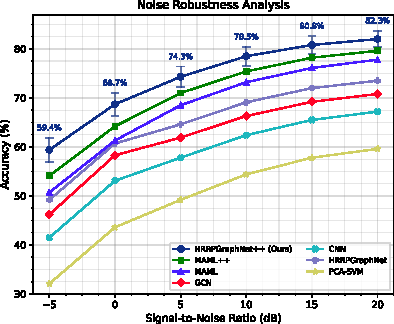
\includegraphics[width=0.5\linewidth]{figures/noise_robust.pdf} % 使用与原文相同的图
    % \fbox{图 3.2: 不同方法在不同SNR下的准确率 (3-way 5-shot) (占位符,同原文 Figure 3)}
    \caption{HRRPGraphNet++及对比方法在不同SNR下的识别准确率变化曲线}
    \label{fig:noise_robustness_chap3}
\end{figure}

接着,针对方法的噪声鲁棒性进行重点评估。本文在3-way 5-shot的设定下,测试了不同方法在不同信噪比(SNR从20dB降至-5dB)条件下的平均识别准确率。结果如图~\ref{fig:noise_robustness_chap3}所示。可以看出,随着SNR的降低,所有方法的性能都出现下降,但HRRPGraphNet++表现出明显更强的鲁棒性。在SNR从20dB降至-5dB的过程中,HRRPGraphNet++的准确率从约91.8\%下降到59.4\%,性能下降相对平缓。相比之下,其他方法的性能下降更为剧烈。例如,在SNR=0dB时,HRRPGraphNet++的准确率约为68.7\%,显著高于MAML++(约64.2\%)、GCN(约58.3\%)和CNN(约53.1\%)。这表明所提的动态图结构和面向噪声的元学习框架能够有效抵抗噪声干扰,在低信噪比条件下保持较好的识别能力。动态图机制可能有助于模型在噪声存在时自适应地调整节点间的依赖关系,关注更可靠的信号成分,而元学习框架则使得模型能够利用少量样本快速适应当前的噪声水平。

% --- 网络结构消融实验图占位符 ---
\begin{figure}[h]
    \centering
    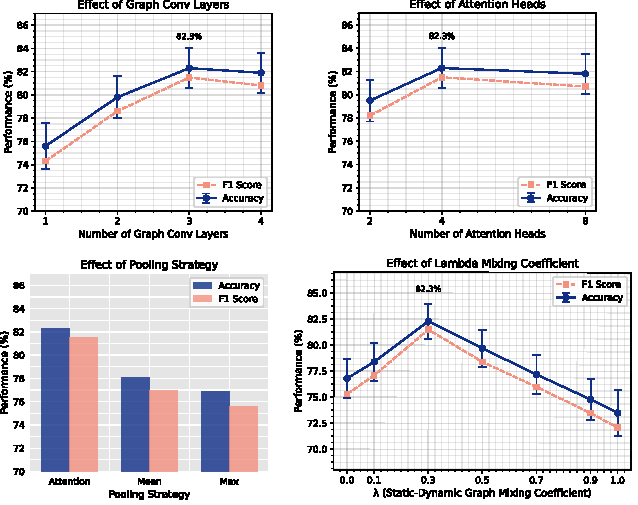
\includegraphics[width=0.8\linewidth]{figures/abla.pdf} % 使用与原文相同的图
    % \fbox{图 3.3: 网络结构消融实验结果 (占位符,同原文 Figure 4)}
    \caption{所提HRRPGraphNet++方法GCN层数、注意力头数、池化策略及混合邻接矩阵中静态与动态成分的融合权重$\lambda$消融结果}
    \label{fig:abla}
\end{figure}

最后,进行消融实验来分析模型各关键组成部分的作用。图~\ref{fig:abla}展示了GNN层数、注意力头数和池化策略对模型性能(3-way 5-shot, SNR=20dB)的影响。结果显示,使用3层GCN时性能最佳,层数过少(1层)或过多(4层)都会导致性能下降,这与GNN中常见的过平滑现象一致。对于动态图构建中的多头注意力机制,使用4个头时效果最好,头数过少(2个)可能无法捕捉足够多样性的关系,头数过多(8个)则可能引入冗余。在池化策略方面,全局注意力池化显著优于全局平均池化和全局最大池化,证明了自适应地关注重要节点对于HRRP图表示学习的重要性。同时,图~\ref{fig:abla}也展示了混合图构建中静态/动态成分融合权重 $\lambda$ 对性能的影响。当 $\lambda=0$ 时(仅使用动态图),性能尚可但不如混合图;当 $\lambda=1$ 时(仅使用静态图),性能显著下降;当 $\lambda$ 取中间值时性能较好,并在 $\lambda=0.3$ 附近达到最优。这验证了所提混合动态图策略的有效性:结合基于物理先验的静态结构和基于数据驱动的动态结构能够取得最佳效果,表明静态先验提供了有用的结构约束,而动态适应性对于捕捉HRRP的复杂特性至关重要。

综合以上实验结果,所提HRRPGraphNet++方法通过结合动态图表示学习和改进的元学习框架,在小样本HRRP识别任务中,尤其是在噪声环境下,展现出了优越的性能和鲁棒性。

\section{本章小结}
\label{sec:noise_summary}

本章针对小样本HRRP雷达目标识别在实际应用中普遍存在的噪声干扰问题,提出了一种基于动态图元学习的鲁棒识别方法HRRPGraphNet++。首先,深入分析了低信噪比条件下噪声对HRRP信号特性及识别性能带来的不利影响,明确了提升噪声鲁棒性的必要性。随后,详细阐述了所提方法的核心组成:一是设计了一种混合动态图构建策略,通过融合基于物理先验的静态连接和基于多头自注意力机制的动态连接为每个HRRP样本生成自适应的图结构表示 $\hat{\mathbf{A}}$;二是构建了一个包含初始特征提取、多层图卷积和全局注意力池化的GNN模块,用于学习图表示;三是将动态图学习与GNN模块嵌入到一个经过改进的面向噪声鲁棒性的元学习框架中,采用了多步内循环更新、多步损失优化、层级学习率和任务级BN统计量等策略,并通过在含噪任务上进行元训练,使模型具备快速适应和鲁棒识别的能力。最后,本章给出了方法的整体流程的详细说明。

仿真实验结果充分验证了HRRPGraphNet++方法的有效性。在小样本识别任务中,该方法在1-shot、5-shot、20-shot下均取得了最优识别准确率。在噪声鲁棒性测试中,HRRPGraphNet++相比于其他基线方法表现出明显更强的抗噪声能力,在SNR从20dB降至-5dB的过程中性能下降更为平缓。消融实验进一步证实了动态图机制以及GNN架构和元学习框架中各改进组件的积极作用。综上所述,本章提出的HRRPGraphNet++方法为解决小样本、噪声环境下的HRRP识别问题提供了一种有效的解决方案,其核心思想是将数据自适应的图结构学习与元学习的快速适应能力相结合,为提升RATR系统在复杂环境下的性能奠定了基础。
